\documentclass{standalone}
\usepackage[utf8]{inputenc}
\usepackage{pgfplots}
\DeclareUnicodeCharacter{2212}{−}
\usepgfplotslibrary{groupplots,dateplot}
\usetikzlibrary{patterns,shapes.arrows}
\pgfplotsset{compat=newest}
\begin{document}
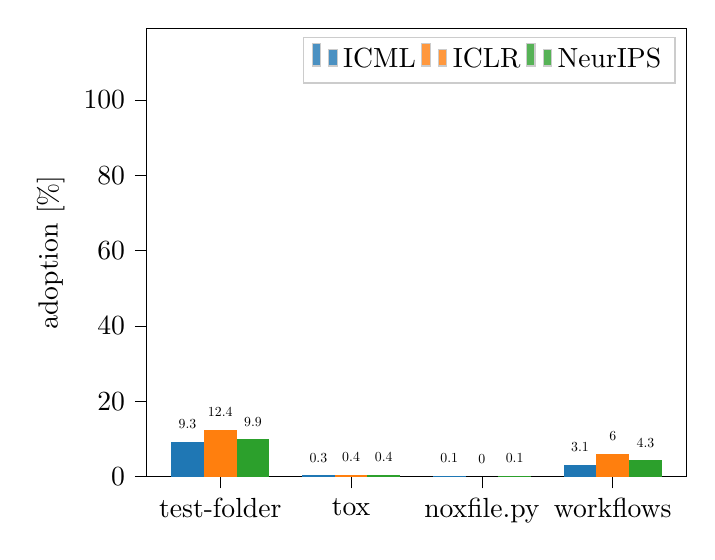
\begin{tikzpicture}

\definecolor{darkgray176}{RGB}{176,176,176}
\definecolor{darkorange25512714}{RGB}{255,127,14}
\definecolor{forestgreen4416044}{RGB}{44,160,44}
\definecolor{lightgray204}{RGB}{204,204,204}
\definecolor{steelblue31119180}{RGB}{31,119,180}

\begin{axis}[
legend cell align={left},
legend columns=3,
legend style={fill opacity=0.8, draw opacity=1, text opacity=1, draw=lightgray204},
tick align=outside,
tick pos=left,
x grid style={darkgray176},
xmin=-0.3125, xmax=3.8125,
xtick style={color=black},
xtick={0.25,1.25,2.25,3.25},
xticklabels={test-folder,tox,noxfile.py,workflows},
y grid style={darkgray176},
ylabel={adoption [\%]},
ymin=0, ymax=119,
ytick style={color=black}
]
\draw[draw=none,fill=steelblue31119180] (axis cs:-0.125,0) rectangle (axis cs:0.125,9.3);
\addlegendimage{ybar,ybar legend,draw=none,fill=steelblue31119180}
\addlegendentry{ICML}

\draw[draw=none,fill=steelblue31119180] (axis cs:0.875,0) rectangle (axis cs:1.125,0.3);
\draw[draw=none,fill=steelblue31119180] (axis cs:1.875,0) rectangle (axis cs:2.125,0.1);
\draw[draw=none,fill=steelblue31119180] (axis cs:2.875,0) rectangle (axis cs:3.125,3.1);
\draw[draw=none,fill=darkorange25512714] (axis cs:0.125,0) rectangle (axis cs:0.375,12.4);
\addlegendimage{ybar,ybar legend,draw=none,fill=darkorange25512714}
\addlegendentry{ICLR}

\draw[draw=none,fill=darkorange25512714] (axis cs:1.125,0) rectangle (axis cs:1.375,0.4);
\draw[draw=none,fill=darkorange25512714] (axis cs:2.125,0) rectangle (axis cs:2.375,0);
\draw[draw=none,fill=darkorange25512714] (axis cs:3.125,0) rectangle (axis cs:3.375,6);
\draw[draw=none,fill=forestgreen4416044] (axis cs:0.375,0) rectangle (axis cs:0.625,9.9);
\addlegendimage{ybar,ybar legend,draw=none,fill=forestgreen4416044}
\addlegendentry{NeurIPS}

\draw[draw=none,fill=forestgreen4416044] (axis cs:1.375,0) rectangle (axis cs:1.625,0.4);
\draw[draw=none,fill=forestgreen4416044] (axis cs:2.375,0) rectangle (axis cs:2.625,0.1);
\draw[draw=none,fill=forestgreen4416044] (axis cs:3.375,0) rectangle (axis cs:3.625,4.3);
\draw (axis cs:0,9.3) ++(0pt,3pt) node[
  scale=0.5,
  anchor=south,
  text=black,
  rotate=0.0
]{9.3};
\draw (axis cs:1,0.3) ++(0pt,3pt) node[
  scale=0.5,
  anchor=south,
  text=black,
  rotate=0.0
]{0.3};
\draw (axis cs:2,0.1) ++(0pt,3pt) node[
  scale=0.5,
  anchor=south,
  text=black,
  rotate=0.0
]{0.1};
\draw (axis cs:3,3.1) ++(0pt,3pt) node[
  scale=0.5,
  anchor=south,
  text=black,
  rotate=0.0
]{3.1};
\draw (axis cs:0.25,12.4) ++(0pt,3pt) node[
  scale=0.5,
  anchor=south,
  text=black,
  rotate=0.0
]{12.4};
\draw (axis cs:1.25,0.4) ++(0pt,3pt) node[
  scale=0.5,
  anchor=south,
  text=black,
  rotate=0.0
]{0.4};
\draw (axis cs:2.25,0) ++(0pt,3pt) node[
  scale=0.5,
  anchor=south,
  text=black,
  rotate=0.0
]{0};
\draw (axis cs:3.25,6) ++(0pt,3pt) node[
  scale=0.5,
  anchor=south,
  text=black,
  rotate=0.0
]{6};
\draw (axis cs:0.5,9.9) ++(0pt,3pt) node[
  scale=0.5,
  anchor=south,
  text=black,
  rotate=0.0
]{9.9};
\draw (axis cs:1.5,0.4) ++(0pt,3pt) node[
  scale=0.5,
  anchor=south,
  text=black,
  rotate=0.0
]{0.4};
\draw (axis cs:2.5,0.1) ++(0pt,3pt) node[
  scale=0.5,
  anchor=south,
  text=black,
  rotate=0.0
]{0.1};
\draw (axis cs:3.5,4.3) ++(0pt,3pt) node[
  scale=0.5,
  anchor=south,
  text=black,
  rotate=0.0
]{4.3};
\end{axis}

\end{tikzpicture}

\end{document}
